\documentclass[10pt]{article}
\usepackage[a4paper,margin=5mm,landscape]{geometry}
\usepackage{blindtext}

\usepackage{multicol}
\usepackage{enumitem}
\usepackage[dvipsnames]{xcolor}
\usepackage{graphicx}
\usepackage{hyperref}



\usepackage[condensed,math]{iwona}

\usepackage[sfdefault,condensed]{roboto}  %% Option 'sfdefault' only if the base font of the document is to be sans serif
\usepackage[T1]{fontenc}


% Marca d'agua
%\usepackage{draftwatermark}
%\SetWatermarkText{Draft}
%\SetWatermarkScale{5}

\setlength{\columnseprule}{.5pt}
\linespread{.95}

\usepackage{titlesec}
\titlespacing{\subsection}{0pc}{3.pt}{1.pt}
\titlespacing{\subsubsection}{0pc}{1.5pt}{1.pt}

\definecolor{mygray}{RGB}{245, 245, 245}
\pagecolor{mygray}

\usepackage{float}

\setlength{\textfloatsep}{1pt}
\setlength{\floatsep}{1pt}
\setlength{\intextsep}{1pt}

\begin{document}
\noindent
{\large{\textbf{\emph{C++ Standard Library Cheat Sheet}}, {\small version 1.0}}	
}

\noindent
{\small  Roberto D. Algarte (2024)}
\par\noindent\rule{\linewidth}{0.4pt}

\scriptsize
\begin{multicols*}{5}

{\color{Blue}
\subsection*{\center{\textsc{notation}}}	

\begin{itemize}[leftmargin=*,topsep=0.25pt]
  \setlength\itemsep{-1.8pt}
	\item \textbf{priority\_queue} @ $<$queue$>$: class ``std::pri\-ori\-ty\_que\-ue'' that belongs to library ``queue''. 
	\item \emph{\textbf{setbase}} @ $<$iomanip$>$: standalone function ``std::setbase'' that belongs to library ``iomanip'';
	\item basic\_ios::\emph{\textbf{good}} @ $<$iostream$>$: member function ``good'' of an object from class ``std::basic\_ios'' that belongs to library ``iostream''; 
	\item Items in lists are alphabetically sorted; 
	\item Section titles are linked to \href{https://en.cppreference.com}{\underline{cppreference.com}} 
\end{itemize}

\par\noindent\rule{155pt}{0.4pt}

}

{\color{Blue}
\subsection*{\href{https://en.cppreference.com/w/cpp/container}{\underline{CONTAINERS}}}	
\noindent
Aggregates of elements that provide element insertion, removal and access.

\subsubsection*{\textsc{Theory} - \emph{Time Complexity}} 
\begin{figure}[H]
\begin{center}
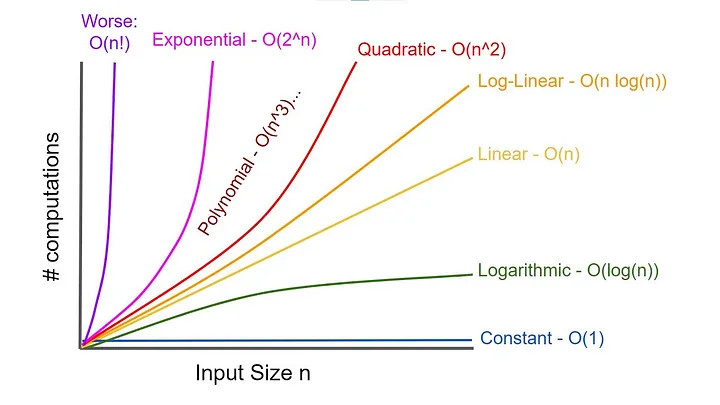
\includegraphics[scale=.21]{complexity.jpg}	
\end{center}
\end{figure}

\subsubsection*{\textsc{Theory} - \emph{Linear Aggregates}} 

\begin{itemize}[leftmargin=*,topsep=0.25pt]
  \setlength\itemsep{-1.8pt}
	\item \emph{Array}: static or dynamic structure whose elements have defined positions and are stored in contiguous memory. Insertion and removal of elements may imply repositioning of other elements or repositioning of the entire structure; 
	\item \emph{Linked list}: dynamic structure whose elements may not be stored contiguously. A node (list element) is composed by a value and one or two references to adjacent nodes. Nodes of a \emph{doubly-linked} list have two references, and of a \emph{singly-linked}, one reference. Insertion and removal don't imply repositioning of other elements;
	\item \emph{Queue}: FIFO dynamic structure with two ends, one for insertion and another for removal; access can be performed on both. In a \emph{double-ended} queue, both ends allow insertion and removal;  
	\item \emph{Stack}: LIFO dynamic structure with one end, in which insertion, deletion and access are performed;
\end{itemize}

\subsubsection*{\textsc{Sequence Containers}} 
\noindent
Containers whose elements can be accessed sequentially and are stored contiguously on the heap memory.

\begin{itemize}[leftmargin=*,topsep=0.25pt]
  \setlength\itemsep{-1.8pt}
	\item \textbf{array} @ $<$array$>$: wrapper for C static arrays;
	\item \textbf{dequeue} @ $<$dequeue$>$: implementation of a double-ended queue. Insertion, removal and access are $O(1)$;
	\item \textbf{forward\_list} @ $<$forward\_list$>$: implementation of a singly-linked list. Insertion and removal are $O(1)$; access is $O(n)$. Provided by $<$forward\_list$>$;  
	\item \textbf{list} @ $<$list$>$: implementation of a doubly-linked list. Insertion and removal are $O(1)$; access is $O(n)$;
	\item \textbf{vector} @ $<$vector$>$: implementation of a dynamic array. Insertion and removal are $O(1)$ at the end, $O(n)$ elsewhere; access is $O(1)$;
\end{itemize}

\subsubsection*{\textsc{Sequence Container Adapters}} 
\noindent
Wrappers created around dequeue to provide other types of aggregates.

\begin{itemize}[leftmargin=*,topsep=0.25pt]
  \setlength\itemsep{-1.8pt}
	\item \textbf{priority\_queue} @ $<$queue$>$: implementation of a queue in which the front element must observe a priority condition (the largest, by default). Insertion and removal are $O(log(n))$;
	\item \textbf{queue} @ $<$queue$>$: implementation of a simple queue;
	\item \textbf{stack} @ $<$stack$>$: implementation of a stack;
\end{itemize}
\noindent

\subsubsection*{\textsc{Associative Containers}} 
\noindent
Containers constituted by (non)primary key sorted elements or pair of (non)primary key-value sorted elements that are  inserted, removed and accessed in $O(log(n))$ time complexity for the worst case.

\begin{itemize}[leftmargin=*,topsep=0.25pt]
  \setlength\itemsep{-1.8pt}
	\item \textbf{map} @ $<$map$>$: constituted by primary key-value elements;
	\item \textbf{multimap} @ $<$map$>$: constituted by non primary key-value elements;  
	\item \textbf{multiset} @ $<$set$>$: constituted by non primary key elements;
	\item \textbf{set} @ $<$set$>$: constituted by primary key elements;
\end{itemize}
\noindent
Each one of these types has its \textbf{unordered\_*} counterpart, whose elements are inserted or removed in $O(1)$, and accessed in $O(n)$ for the worst case. 




\subsubsection*{\textsc{Main functions}} 
\noindent

\begin{itemize}[leftmargin=*,topsep=0.25pt]
  \setlength\itemsep{-1.8pt}
	\item container::\emph{\textbf{clear}} @ $<$container$>$: empties the container;
	\item container::\emph{\textbf{emplace\_back}} @ $<$container$>$: performs a container::\emph{\textbf{emplace}} at the end iterator;
	\item container::\emph{\textbf{emplace\_front}} @ $<$container$>$: performs a container::\emph{\textbf{emplace}} at the begin iterator;
	\item container::\emph{\textbf{emplace}} @ $<$container$>$: creates and inserts an object before a specified iterator and returns the interator of this inserted object;
	\item container::\emph{\textbf{erase}} @ $<$container$>$: deletes an element whith a specified iterator or range;
	\item container::\emph{\textbf{insert}} @ $<$container$>$: inserts a copy of an object before a specified iterator and returns the interator of this inserted object;
	\item container::\emph{\textbf{push\_back}} @ $<$container$>$: performs a container::\emph{\textbf{insert}} at the end iterator;
	\item container::\emph{\textbf{push\_front}} @ $<$container$>$: performs a container::\emph{\textbf{insert}} at the begin iterator;
\end{itemize}
\noindent


}



\par\noindent\rule{155pt}{0.4pt}

{\color{Blue}
\subsection*{\href{https://en.cppreference.com/w/cpp/io}{\underline{I/O STREAMS}}}	
\noindent
Streams enable flow of data to be written (output) or to be read (input). Output streams can be buffered or not.
The \emph{extractor operator} $<<$ when applied to input streams performs formatted input while the \emph{insertion operator} $>>$ applied to output streams performs formatted output. 

\subsubsection*{\textsc{Console Streams}} 
\begin{itemize}[leftmargin=*,topsep=0.25pt]
  \setlength\itemsep{-1.8pt}
	\item \textbf{cerr} @ $<$iostream$>$: wrapper around the standard C stream stderr, which writes data to the console;
	\item \textbf{cin} @ $<$iostream$>$: wrapper around the standard C stream stdin, which reads data from the console;
	\item \textbf{cout} @ $<$iostream$>$: wrapper around the standard C stream stdout, which writes data to the console and is buffered;
\end{itemize}

\subsubsection*{\textsc{String Streams}}
\noindent
Streams that enable flow of outputted or inputted strings.

\begin{itemize}[leftmargin=*,topsep=0.25pt]
  \setlength\itemsep{-1.8pt}
	\item \textbf{basic\_istringstream} @ $<$sstream$>$: provides high level string input formatting;
	\item \textbf{basic\_ostringstream} @ $<$sstream$>$: provides high level string output formatting;
	\item \textbf{basic\_stringstream} @ $<$sstream$>$: provides high level string input/output formatting;
\end{itemize}


\subsubsection*{\textsc{File Streams}} 
\noindent
Streams that enable flow of outputted or inputted data to or from files.

\begin{itemize}[leftmargin=*,topsep=0.25pt]
  \setlength\itemsep{-1.8pt}
	\item \textbf{basic\_ifstream} @ $<$fstream$>$: provides high level file input formatting;
	\item \textbf{basic\_fstream} @ $<$fstream$>$: provides high level file input/output formatting;
	\item \textbf{basic\_ofstream} @ $<$fstream$>$: provides high level file output formatting;
\end{itemize}

\subsubsection*{\textsc{Aliases}} 
\begin{itemize}[leftmargin=*,topsep=0.25pt]
  \setlength\itemsep{-1.8pt}
	\item \textbf{ifstream} $=$ \textbf{basic\_ifstream}<char>;
	\item \textbf{istringstream} $=$ \textbf{basic\_istringstream}<char>;
	\item \textbf{fstream} $=$ \textbf{basic\_fstream}<char>;
	\item \textbf{ofstream} $=$ \textbf{basic\_ofstream}<char>;
	\item \textbf{ostringstream} $=$ \textbf{ba\-sic\_o\-string\-stream}\-<char>;
	\item \textbf{stringstream} $=$ \textbf{basic\_stringstream}<char>;
\end{itemize}


\subsubsection*{\textsc{Manipulators and Formatters}} 
\begin{itemize}[leftmargin=*,topsep=0.25pt]
  \setlength\itemsep{-1.8pt}
	\item \textbf{boolalpha} @ $<$ios$>$: sets text values for booleans;
	\item \textbf{defaultfloat} @ $<$ios$>$: outputs floats as default;
	\item \emph{\textbf{endl}} @ $<$ostream$>$: inserts a line break and flushes the buffer; 
	\item \emph{\textbf{ends}} @ $<$iomanip$>$: inserts a null character; 
	\item \textbf{fixed} @ $<$ios$>$: outputs floats in fixed width;
	\item \emph{\textbf{flush}} @ $<$ostream$>$: flushes the stream buffer; 
	\item \emph{\textbf{get\_money}} @ $<$iomanip$>$: parse value as currency; 
	\item \emph{\textbf{get\_time}} @ $<$iomanip$>$: parses value as a datetime; 
	\item \emph{\textbf{getline}} @ $<$string$>$:  reads a line from input stream setting the reading pointer to the new line. By default, lines are separated by line breaks;
	\item \textbf{hexfloat} @ $<$ios$>$: outputs floats in hex notation;
	\item \textbf{hex} @ $<$ios$>$: outputs in base 16;
	\item \textbf{left} @ $<$ios$>$: sets left as the output position of the fill char;
	\item \textbf{oct} @ $<$ios$>$: outputs in base 8;
	\item \emph{\textbf{put\_money}} @ $<$iomanip$>$: sets values to currency; 
	\item \emph{\textbf{put\_time}} @ $<$iomanip$>$: outputs a \textbf{std:tm} object with specified format; 
	\item \emph{\textbf{quoted}} @ $<$iomanip$>$: correctly reads and writes strings with quotes; 
	\item \textbf{right} @ $<$ios$>$: sets right as the output position of the fill char;
	\item \textbf{scientific} @ $<$ios$>$: outputs floats in scientific notation;
	\item \emph{\textbf{setbase}} @ $<$iomanip$>$: sets the output base; 
	\item \emph{\textbf{setfill}} @ $<$iomanip$>$:sets a fill character instead of white space; 
	\item \emph{\textbf{setprecision}} @ $<$iomanip$>$: sets the precision of floats; 
	\item \emph{\textbf{setw}} @ $<$iomanip$>$: sets the output width for the text; 
	\item \textbf{showbase} @ $<$ios$>$: enables base prefix in numbers;
	\item \textbf{showpoint} @ $<$ios$>$: enables decimal point in numbers;
	\item \textbf{showpos} @ $<$ios$>$: pre-print a $+$ in nonnegative numbers;
	\item \textbf{skipws} @ $<$ios$>$: skips white spaces;
	\item \textbf{unitbuf} @ $<$ios$>$: sets buffer flushing for every output operation;
	\item \textbf{uppercase} @ $<$ios$>$: sets the output chars to be uppercased;
\end{itemize}

\subsubsection*{\textsc{States}} 
\begin{itemize}[leftmargin=*,topsep=0.25pt]
  \setlength\itemsep{-1.8pt}
	\item basic\_ios::\emph{\textbf{bad}} @ $<$iostream$>$: stream is in a non recoverable error state;
	\item basic\_ios::\emph{\textbf{clear}} @ $<$iostream$>$: refresh the state of the stream;
	\item basic\_ios::\emph{\textbf{eof}} @ $<$iostream$>$: reading pointer arrived at the end of file;
	\item basic\_ios::\emph{\textbf{fail}} @ $<$iostream$>$: stream is in a recoverable error state;
	\item basic\_ios::\emph{\textbf{good}} @ $<$iostream$>$: stream is fine an can be read or written to;
\end{itemize}


}

\par\noindent\rule{155pt}{0.4pt}

{\color{Blue}
\subsection*{\href{https://en.cppreference.com/w/cpp/iterator}{\underline{ITERATORS}}}	
\noindent
Pointer-like types created to implement the iterator pattern in STL. The iterator pattern states that aggregate structures and element-accessing functions should be decoupled.

\subsubsection*{\textsc{Iteratable Aggregates}} 
\noindent
All types of STL containers, C arrays, input and output streams.

\subsubsection*{\textsc{Concepts}} 
\begin{itemize}[leftmargin=*,topsep=0.25pt]
  \setlength\itemsep{-1.8pt}
	\item \textbf{bidirectional\_iterator} @ $<$iterator$>$: a \textbf{for\-ward\_ite\-ra\-tor} able to traverse backwards; 
	\item \textbf{contiguous\_iterator} @ $<$iterator$>$: a specific \textbf{ran\-dom\_ac\-cess\_i\-te\-ra\-tor} that traverses elements stored contiguously in memory (e.g. vector). 
	\item \textbf{forward\_iterator} @ $<$iterator$>$: an \textbf{input\_iterator} that has equality comparison and multi-pass, which means that it can traverse multiple times the elements of an aggregate (e.g. containers); 
	\item \textbf{input\_iterator} @ $<$iterator$>$: a type that can be both pre- and post-incremented, related to a given structures whose values can be read (e.g. input streams);
	\item \textbf{istream\_iterator} @ $<$iterator$>$: a specific type of \textbf{in\-put\_i\-te\-ra\-tor} that reads from an input stream;
	\item \textbf{ostream\_iterator} @ $<$iterator$>$: a specific type of \textbf{out\-put\_i\-te\-ra\-tor} that writes to an output stream;
	\item \textbf{output\_iterator} @ $<$iterator$>$: a type that can be both pre- and post-incremented, related to a given structure to which values can be written (e.g. output streams);
	\item \textbf{random\_access\_iterator} @ $<$iterator$>$: a \textbf{bidirectional\_iterator} that supports subscripting with $O(1)$ time access to elements; 
\end{itemize}

\subsubsection*{\textsc{Range Functions}} 
\begin{itemize}[leftmargin=*,topsep=0.25pt]
  \setlength\itemsep{-1.8pt}
	\item  \emph{\textbf{begin}} @ $<$iterator$>$: returns the first element read-write iterator. The function \emph{\textbf{cbegin}} returns the read-only version;
	\item  \emph{\textbf{end}} @ $<$iterator$>$: returns the one-past-the-last element read-write iterator. The function \emph{\textbf{cend}} returns the read-only version;
	\item  \emph{\textbf{rbegin}} @ $<$iterator$>$: returns the first element read-write reverse iterator. The function \emph{\textbf{crbegin}} returns the read-only version;
	\item  \emph{\textbf{rend}} @ $<$iterator$>$: returns the one-past-the-last element read-write reverse iterator. The function \emph{\textbf{crend}} returns the read-only version;
	\item  \emph{\textbf{ranges::reverse\_view}} @ $<$ranges$>$: returns the reversed range of its argument;
\end{itemize}

\subsubsection*{\textsc{Adapters}} 
\noindent
Iterator wrappers created to encapsulate some important iterator-related functionalities. 
\begin{itemize}[leftmargin=*,topsep=0.25pt]
  \setlength\itemsep{-1.8pt}
	\item \textbf{back\_insert\_iterator} @ $<$iterator$>$: performs back insertion of elements. This adapter can be created by the helper function \emph{\textbf{back\_inserter}};
	\item \textbf{front\_insert\_iterator} @ $<$iterator$>$: performs front insertion of elements. This adapter can be created by the helper function \emph{\textbf{front\_inserter}};
	\item \textbf{insert\_iterator} @ $<$iterator$>$: performs insertion of element at a specified position. This adapter can be created by the helper function \emph{\textbf{inserter}};
	\item \textbf{move\_iterator} @ $<$iterator$>$: performs move of elements from one aggregate to another. This adapter can be created by the helper function \emph{\textbf{make\_move\_iterator}};
	\item \textbf{reverse\_iterator} @ $<$iterator$>$: performs reverse order traversal. This adapter can be created by the helper function \emph{\textbf{make\_reverse\_iterator}};
\end{itemize}

\subsubsection*{\textsc{Operations}} 
\begin{itemize}[leftmargin=*,topsep=0.25pt]
  \setlength\itemsep{-1.8pt}
	\item  \emph{\textbf{advance}} @ $<$iterator$>$: advances an iterator by a given distance;
	\item  \emph{\textbf{data}} @ $<$iterator$>$: returns the pointer to the given sequence container;
	\item  \emph{\textbf{distance}} @ $<$iterator$>$: returns the number of elements between two iterators in which the first is included and last excluded;
	\item  \emph{\textbf{empty}} @ $<$iterator$>$: checks whether the given range empty;
	\item  \emph{\textbf{next}} @ $<$iterator$>$: increments an iterator returning it;
	\item  \emph{\textbf{prev}} @ $<$iterator$>$: decrements an iterator returning it;
\end{itemize}
}

\par\noindent\rule{155pt}{0.4pt}

{\color{Blue}
\subsection*{\href{https://en.cppreference.com/w/cpp/algorithm}{\underline{ALGORITHMS}}}	
\noindent  
Collection of libraries that handle ranges of elements providing a variety of functionalities like searching, counting, sorting, partitioning and transforming.


\subsubsection*{\textsc{Numeric Functions}} 
\begin{itemize}[leftmargin=*,topsep=0.25pt]
  \setlength\itemsep{-1.8pt}
	\item  \emph{\textbf{accumulate}} @ $<$numeric$>$: sums up or folds sequentially a range of elements;
		\item  \emph{\textbf{adjacent\_difference}} @ $<$numeric$>$: computes the difference between two adjacent values in a range storing them in the original range;
	\item  \emph{\textbf{inner\_product}} @ $<$numeric$>$: returns the inner product of two ranges;
	\item  \emph{\textbf{iota}} @ $<$numeric$>$: fills a range with successive increments of the starting value;
	\item  \emph{\textbf{inclusive\_scan}} @ $<$numeric$>$: sums up or folds the elements from beginning to each element position, storing each result in the original range, according to the execution policy;
	\item  \emph{\textbf{partial\_sum}} @ $<$numeric$>$: sums up or folds sequentially the elements from beginning to each element position, storing each result in the original range;
\item  \emph{\textbf{reduce}} @ $<$numeric$>$: sums up or folds a range of elements according to the execution policy (it may reorder the elements);
	\item  \emph{\textbf{transform\_reduce}} @ $<$numeric$>$: re-implementation of \emph{\textbf{inner\_product}} with execution policy support;
	\end{itemize}


\subsubsection*{\textsc{Sorting Functions}} 
\begin{itemize}[leftmargin=*,topsep=0.25pt]
  \setlength\itemsep{-1.8pt}
	\item  \emph{\textbf{is\_sorted\_until}} @ $<$algorithm$>$: finds the largest sub-range inside a range whose elements are non-descending ordered;
	\item  \emph{\textbf{is\_sorted}} @ $<$algorithm$>$: checks if the elements are non-descending ordered;
	\item  \emph{\textbf{nth\_element}} @ $<$algorithm$>$: rearranges the elements in such a way that the value at the position n corresponds to the n-th element of the sorted range;
	\item  \emph{\textbf{partial\_sort\_copy}} @ $<$algorithm$>$: copies an ascending sorts from begin until a specified position of a range to another range;
	\item  \emph{\textbf{partial\_sort}} @ $<$algorithm$>$: sorts a range in ascending order from begin until a specified position;
	\item  \emph{\textbf{sort}} @ $<$algorithm$>$: sorts a range in ascending order;
	\item  \emph{\textbf{stable\_sort}} @ $<$algorithm$>$: sorts a range in ascending order such that the original order of equally indexed elements of multi-associative containers is preserved;
\end{itemize}

\subsubsection*{\textsc{Main Modifying Functions}} 
\begin{itemize}[leftmargin=*,topsep=0.25pt]
  \setlength\itemsep{-1.8pt}
	\item  \emph{\textbf{copy\_backward}} @ $<$algorithm$>$: copies a range, from end to beginning, to another range;
	\item  \emph{\textbf{copy\_if}} @ $<$algorithm$>$: copies a range, from beginning to end, to another range that obey a predicate;
	\item  \emph{\textbf{copy\_n}} @ $<$algorithm$>$: copies n elements of a range, from beginning to end, to another range;
	\item  \emph{\textbf{copy}} @ $<$algorithm$>$: copies a range, from beginning to end, to another range;
	\item  \emph{\textbf{fill}} @ $<$algorithm$>$: copies a specified value to all elements in a range;
	\item  \emph{\textbf{generate}} @ $<$algorithm$>$: populates a range through a callable object;
	\item  \emph{\textbf{is\_permutation}} @ $<$algorithm$>$: checks whether a range is a permutation of another range;
	\item  \emph{\textbf{iter\_swap}} @ $<$algorithm$>$: swaps values pointed by two iterators;
	\item  \emph{\textbf{move\_backward}} @ $<$algorithm$>$: moves the elements of a range, from end to beginning, to another range. Afterwards, the elements of the source range are left in undefined state;
	\item  \emph{\textbf{move}} @ $<$algorithm$>$: moves the elements of a range, from beginning to end, to another range. Afterwards, the elements of the source range are left in undefined state;
	\item  \emph{\textbf{next\_permutation}} @ $<$algorithm$>$: performs the next permutation in a range returning false if it's the last permutation. The reference is the sorted range;
	\item  \emph{\textbf{partition\_copy}} @ $<$algorithm$>$: copies the elements of a range to two other ranges so that one target range receives elements that obey a predicate and the other receives the remaining elements;
	\item  \emph{\textbf{partition}} @ $<$algorithm$>$: reorders the elements of a range so that elements that obey a predicate precede the elements that don't. The relative order of the elements may not be preserved;
	\item  \emph{\textbf{prev\_permutation}} @ $<$algorithm$>$: performs the previous permutation in a range returning true if it's the first permutation. The reference is the sorted range;
	\item  \emph{\textbf{remove\_copy\_if}} @ $<$algorithm$>$: copies all the elements of a range to another that disobey a predicate; 
	\item  \emph{\textbf{remove\_copy}} @ $<$algorithm$>$: copies all the elements of a range to another that are different from a value;
	\item  \emph{\textbf{remove\_if}} @ $<$algorithm$>$: removes all the elements of a range that obey to a predicate; 
	\item  \emph{\textbf{remove}} @ $<$algorithm$>$: removes all the elements of a range equal to a value;
	\item  \emph{\textbf{replace\_copy\_if}} @ $<$algorithm$>$: copies all the elements of a range to another range replacing the elements that obey a predicate by a specified value;
	\item  \emph{\textbf{replace\_copy}} @ $<$algorithm$>$: copies all the elements of a range to another range replacing the elements equal to a given value by a specified value;
	\item  \emph{\textbf{replace\_if}} @ $<$algorithm$>$: replaces all the elements that obey a predicate by a specified value;
	\item  \emph{\textbf{replace}} @ $<$algorithm$>$: replaces all the elements of a range equal to a given value by a specified value;
	\item  \emph{\textbf{reverse\_copy}} @ $<$algorithm$>$: copies a range of size n, from end to beginning, to another range of size n;
	\item  \emph{\textbf{rotate\_copy}} @ $<$algorithm$>$: copies a left rotation of a range of elements to another range;
	\item  \emph{\textbf{rotate}} @ $<$algorithm$>$: performs a left rotation of a range of elements;
	\item  \emph{\textbf{sample}} @ $<$algorithm$>$: given a random number generator like {\textbf{mt19937}}, selects n elements of a given range and copies them to an output iterator;
	\item  \emph{\textbf{shuffle}} @ $<$algorithm$>$: given a random number generator like {\textbf{mt19937}}, shuffles the elements of a given range;
	\item  \emph{\textbf{stable\_partition}} @ $<$algorithm$>$: performs the same actions of  \emph{\textbf{partition}}, but preserves the relative order of elements. 
	\item  \emph{\textbf{swap\_ranges}} @ $<$algorithm$>$: swaps every element of a n-distance range with another n-distance range;
	\item  \emph{\textbf{swap}} @ $<$algorithm$>$: moves the values of two variables to one another;
\end{itemize}

\subsubsection*{\textsc{Main Non-modifying Functions}} 
\begin{itemize}[leftmargin=*,topsep=0.25pt]
  \setlength\itemsep{-1.8pt}
	\item  \emph{\textbf{adjacent\_find}} @ $<$algorithm$>$: finds the first occurrence of two consecutive equal elements;
	\item  \emph{\textbf{binary\_search}} @ $<$algorithm$>$: finds the first element of a sorted range equal to a value;  
	\item  \emph{\textbf{clamp}} @ $<$algorithm$>$: given an upper and lower boundary and a value n, returns n if it is inside the range; otherwise returns the nearest boundary;  
	\item  \emph{\textbf{count\_if}} @ $<$algorithm$>$: returns the frequency of a value in a range that obey a predicate;
	\item  \emph{\textbf{count}} @ $<$algorithm$>$: returns the frequency of a value in a range; 
	\item  \emph{\textbf{equal}} @ $<$algorithm$>$: compares two ranges element by element, obeying or not a predicate;  
	\item  \emph{\textbf{find\_first\_if}} @ $<$algorithm$>$: finds the first element of a range that also belongs to another range;  
	\item  \emph{\textbf{find\_if}} @ $<$algorithm$>$: finds the first element of a range that obey a predicate;
	\item  \emph{\textbf{find}} @ $<$algorithm$>$: finds the first element of a range equal to a value; 
	\item  \emph{\textbf{for\_each}} @ $<$algorithm$>$: applies a callable object to the elements of a range;
	\item  \emph{\textbf{max}} @ $<$algorithm$>$: returns the biggest value between two values or in a initializer list;  
	\item  \emph{\textbf{min}} @ $<$algorithm$>$: returns the smallest value between two values or in a initializer list;  
	\item  \emph{\textbf{search}} @ $<$algorithm$>$: finds the first range of elements equal to a specified range of elements;  
	\item  \emph{\textbf{transform}} @ $<$algorithm$>$: transforms each element of one or more ranges according to a predicate (one or more parameters) and populate another range with the results;  
\end{itemize}

\subsubsection*{\textsc{Execution Policies}} 
\begin{itemize}[leftmargin=*,topsep=0.25pt]
  \setlength\itemsep{-1.8pt}
	\item  {\textbf{execution::par}} @ $<$execution$>$: the algorithm will run parallelized in multiple threads;
\item  {\textbf{execution::par\_unseq}} @ $<$execution$>$: the algorithm may run with vectorization (single instruction in multiple data) in multiple threads; 
	\item  {\textbf{execution::seq}} @ $<$execution$>$: the algorithm will run sequentially in a single thread;
\item  {\textbf{execution::unseq}} @ $<$execution$>$: the algorithm may run with vectorization (single instruction in multiple data) in a single thread.

\end{itemize}



}

\par\noindent\rule{155pt}{0.4pt}

{\color{Blue}
\subsection*{\href{https://en.cppreference.com/w/cpp/thread}{\underline{CONCURRENCY}}}	
\noindent
Collection of libraries that provide functionalities and structures for concurrent programming.

\subsubsection*{\textsc{Theory} - \emph{Basics}} 
\begin{itemize}[leftmargin=*,topsep=0.25pt]
  \setlength\itemsep{-1.8pt}
	\item  \emph{atomic type}: a type whose operations are immune to data races;
	\item  \emph{condition variable}: flag that notifies a state to multiple threads;  
	\item  \emph{data race}: simultaneous thread accesses to shared resources;
	\item  \emph{deadlock}: threads A and B respectively lock resources 1 and 2 and respectively wait for 2 and 1 to be released;
	\item  \emph{mutex}: flag that notifies multiple threads whether to stop or resume execution; 
	\item  \emph{process}: a computer program in execution;
	\item  \emph{thread}: smallest unit of execution within a process;
\end{itemize}

\subsubsection*{\textsc{Atomic Types}} 
\begin{itemize}[leftmargin=*,topsep=0.25pt]
  \setlength\itemsep{-1.8pt}
	\item  \emph{\textbf{atomic}} @ $<$atomic$>$: atomic class template for boolean, integral and floating point types;
	\item  \emph{\textbf{atomic\_ref}} @ $<$atomic$>$: enables atomic operations on non-atomic objects: 
\end{itemize}


\subsubsection*{\textsc{Threads}}
\begin{itemize}[leftmargin=*,topsep=0.25pt]
  \setlength\itemsep{-1.8pt}
	\item  {\textbf{jthread}} @ $<$thread$>$: class providing thread functionalities that automatically joins on destruction;
	\item  \emph{\textbf{this\_thread::get\_id}} @ $<$thread$>$: returns the id of the current thread;
	\item  \emph{\textbf{this\_thread::sleep\_for}} @ $<$thread$>$: stops the execution of the current thread for at least a specified duration;
	\item  {\textbf{thread}} @ $<$thread$>$: class providing thread functionalities;
  \item  thread::\emph{\textbf{detach}} @ $<$thread$>$: parent thread keeps running and doesn't call terminate on child thread;
  \item  thread::\emph{\textbf{join}} @ $<$thread$>$: parent thread stops running to wait for child thread to end;
	\item  thread::\emph{\textbf{hardware\_concurrency}} @ $<$thread$>$: returns the maximum number of system's concurrent threads;
\end{itemize}


\subsubsection*{\textsc{Tasks}}
\noindent
Provides functionalities for obtaining values asynchronously (e.g. returning a value from a child thread to a parent thread).
\begin{itemize}[leftmargin=*,topsep=0.25pt]
  \setlength\itemsep{-1.8pt}
	\item  \emph{\textbf{async}} @ $<$future$>$: executes a specified function asynchronously and returns a \textbf{future};
	\item  {\textbf{future}} @ $<$future$>$: class that waits and returns the value stored asynchronously by its correspondent \textbf{promise};
	\item  {\textbf{promise}} @ $<$future$>$: class that provides a way to store a value asynchronously;
	\item  {\textbf{shared\_future}} @ $<$future$>$: a future whose copies are related to the same \textbf{promise} and then can be dispatched to different threads;
\end{itemize}


\subsubsection*{\textsc{Mutual Exclusions}}
\noindent
Provides functionalities to avoid multiple threads to simultaneously access shared resources (data races).
\begin{itemize}[leftmargin=*,topsep=0.25pt]
  \setlength\itemsep{-1.8pt}
\item  {\textbf{adopt\_lock}} @ $<$mutex$>$: parameter for {\textbf{shared\_lock}} or {\textbf{unique\_lock}} to specify that the lock on the mutex was already performed.
	\item  {{\textbf{condition\_variable\_any}}} @ $<$condition\_variable$>$: provides a condition variable associated with any lock type.
	\item  {{\textbf{condition\_variable}}} @ $<$condition\_variable$>$: provides a condition variable associated with a {\textbf{unique\_lock}}.
\item  {\textbf{defer\_lock}} @ $<$mutex$>$: parameter for {\textbf{shared\_lock}} or {\textbf{unique\_lock}} to specify not to lock the mutex at the construction.
	\item  \textbf{lock\_guard} @ $<$mutex$>$: locks a \textbf{mutex} from the point where it is defined and automatically unlocks it on scope exit or exception throw.
	\item  {{\textbf{unique\_lock}}} @ $<$mutex$>$: locks a \textbf{mutex} from the point where it is defined and automatically unlocks it on scope exit or exception throw. It also allows manual unlocking and locking at specific points.
	\item  {\textbf{mutex}} @ $<$mutex$>$: provides simple mutual exclusion functionalities;
	 \item  mutex::\emph{\textbf{lock}} @ $<$thread$>$: tries to lock the mutex until it succeeds;
	 \item  mutex::\emph{\textbf{try\_lock}} @ $<$thread$>$: tries to lock the mutex and returns true or false;
\item  {\textbf{scope\_lock}} @ $<$mutex$>$: it is the \textbf{lock\_guard} version for simultaneous locking of more than one mutex.
	\item  {\textbf{shared\_lock}} @ $<$shared\_mutex$>$: locks a \textbf{shared\_mutex} from the point where it is defined and automatically unlocks it on scope exit or exception throw. It also allows manual unlocking and locking at specific points..
	\item  \textbf{shared\_mutex} @ $<$shared\_mutex$>$: a type of mutex in which while it is unique-locked, it cannot be unique or shared-locked; while shared-locked, it can be shared-locked but not unique-locked.
\end{itemize}

\subsubsection*{\textsc{Supported Task Functions}} 
\noindent
Function objects (functors), lambdas, variadic templates and member functions; 

}

\par\noindent\rule{155pt}{0.4pt}


{\color{Blue}
\subsection*{\href{https://en.cppreference.com/w/cpp/memory}{\underline{SMART POINTERS}}}	
\noindent
Wrappers around raw pointers with automatic heap memory deallocation allowing different types of ownership.

\subsubsection*{\textsc{Categories}} 
\begin{itemize}[leftmargin=*,topsep=0.25pt]
  \setlength\itemsep{-1.8pt}
	\item  {\textbf{shared\_ptr}} @ $<$memory$>$: smart pointer in which copy is enabled. The number of copies is registered;
	\item  {\textbf{unique\_ptr}} @ $<$memory$>$: smart pointer in which copy is disabled;
	\item  {\textbf{weak\_ptr}} @ $<$memory$>$: smart pointer in which copy is enabled. The number of copies is not registered;
\end{itemize}

\subsubsection*{\textsc{Helper Functions}} 
\begin{itemize}[leftmargin=*,topsep=0.25pt]
  \setlength\itemsep{-1.8pt}
	\item  \emph{\textbf{make\_shared}} @ $<$memory$>$: creates a \textbf{shared\_ptr} from a specified type and object;
	\item  \emph{\textbf{make\_unique}} @ $<$memory$>$: creates a \textbf{unique\_ptr} from a specified type and object;
\end{itemize}

\subsubsection*{\textsc{Function Parameters}} 
\begin{itemize}[leftmargin=*,topsep=0.25pt]
  \setlength\itemsep{-1.8pt}
	\item  \emph{\textbf{f(unique\_ptr<T> ptr)}}: caller must pass the parameter by moving it (ownership transference);
	\item  \emph{\textbf{f(unique\_ptr<T> \&ptr)}}: function can change pointer and object states;
	\item  \emph{\textbf{f(shared\_ptr<T> ptr)}}: another \textbf{shared\_ptr} to the object will be created;
	\item  \emph{\textbf{f(shared\_ptr<T> \&ptr)}}: function can change pointer and object states;
\end{itemize}

}

\par\noindent\rule{155pt}{0.4pt}

{\color{Blue}
\subsection*{\href{https://en.cppreference.com/w/cpp/string}{\underline{STRINGS}}}	
\noindent
Collection of libraries that provide functionalities and structures for handling strings.

\subsubsection*{\textsc{Basic Strings}} 
\begin{itemize}[leftmargin=*,topsep=0.25pt]
  \setlength\itemsep{-1.8pt}
	\item  {\textbf{basic\_string}} @ $<$string$>$: sequence of char type objects stored contiguously in memory;
	\item  {\textbf{basic\_string\_view}} @ $<$string$>$: wrapper around a constant reference to \textbf{basic\_string};
\end{itemize}


\subsubsection*{\textsc{Aliases}} 
\begin{itemize}[leftmargin=*,topsep=0.25pt]
  \setlength\itemsep{-1.8pt}
	\item \textbf{string} $=$ \textbf{basic\_string}<char>;
	\item \textbf{string\_view} $=$ \textbf{basic\_string\_view}<char>;
	\item \textbf{wstring} $=$ \textbf{basic\_string}<wchar\_t>;
	\item \textbf{wstring\_view} $=$ \textbf{basic\_string\_view}<wchar\_t>;
\end{itemize}

\subsubsection*{\textsc{Character Manipulation}} 
\begin{itemize}[leftmargin=*,topsep=0.25pt]
  \setlength\itemsep{-1.8pt}
\item  \emph{\textbf{isalnum}} @ $<$cctype$>$: checks if a character is alphanumeric;
\item  \emph{\textbf{isalpha}} @ $<$cctype$>$: checks if a character is alphabetic;
\item  \emph{\textbf{isblank}} @ $<$cctype$>$: checks if a character is a blank character;
\item  \emph{\textbf{iscntrl}} @ $<$cctype$>$: checks if a character is a control character;
\item  \emph{\textbf{isdigit}} @ $<$cctype$>$: checks if a character is a digit;
\item  \emph{\textbf{isgraph}} @ $<$cctype$>$: checks if a character is a graphical character;
\item  \emph{\textbf{islower}} @ $<$cctype$>$: checks if a character is lowercase;
\item  \emph{\textbf{isprint}} @ $<$cctype$>$: checks if a character is a printing character;
\item  \emph{\textbf{ispunct}} @ $<$cctype$>$: checks if a character is a punctuation character;
\item  \emph{\textbf{isspace}} @ $<$cctype$>$: checks if a character is a space character;
\item  \emph{\textbf{isupper}} @ $<$cctype$>$: checks if a character is an uppercase character;
\item  \emph{\textbf{isxdigit}} @ $<$cctype$>$: checks if a character is a hexadecimal character;
\item  \emph{\textbf{tolower}} @ $<$cctype$>$: converts a character to lowercase;
\item  \emph{\textbf{toupper}} @ $<$cctype$>$: converts a character to uppercase;
\end{itemize}


\subsubsection*{\textsc{Conversions}} 
\begin{itemize}[leftmargin=*,topsep=0.25pt]
  \setlength\itemsep{-1.8pt}
\item  \emph{\textbf{stod}} @ $<$string$>$: converts a string to a double
\item  \emph{\textbf{stof}} @ $<$string$>$: converts a string to a float
\item  \emph{\textbf{stoi}} @ $<$string$>$: converts a string to a signed integer
\item  \emph{\textbf{stold}} @ $<$string$>$: converts a string to a long double
\item  \emph{\textbf{stoll}} @ $<$string$>$: converts a string to a signed long long
\item  \emph{\textbf{stol}} @ $<$string$>$: converts a string to a signed long
\item  \emph{\textbf{stoull}} @ $<$string$>$: converts a string to an unsigned long long
\item  \emph{\textbf{stoul}} @ $<$string$>$: converts a string to an unsigned long
\item  \emph{\textbf{to\_string}} @ $<$string$>$: converts an integral or floating-point value to string
\item  \emph{\textbf{to\_wstring}} @ $<$string$>$: converts an integral or floating-point value to wstring
\end{itemize}

\par\noindent\rule{155pt}{0.4pt}

{\color{Blue}
\subsection*{\href{https://en.cppreference.com/w/cpp/utility}{\underline{UTILITIES}}}	
\noindent
Miscellaneous functionalities and structures.

\subsubsection*{\textsc{Date and Time}} 
\begin{itemize}[leftmargin=*,topsep=0.25pt]
  \setlength\itemsep{-1.8pt}
\item  {\textbf{chrono::system\_clock}} @ $<$chrono$>$: represents the system's real time wall clock; 
\item  {\textbf{chrono::steady\_clock}} @ $<$chrono$>$: represents the system's clock since last boot; 
\item  {\textbf{chrono::time\_point}} @ $<$chrono$>$: represents a point in time; 
\item  {\textbf{chrono::duration}} @ $<$chrono$>$: time duration; 
\item  {\textbf{chrono::hh\_mm\_ss}} @ $<$chrono$>$: splits a \textbf{chrono::duration} in hours, minutes and seconds since midnight;
\item  {\textbf{time\_t}} @ $<$ctime$>$: time type that supports arithmetic operations;
\item  \emph{\textbf{to\_time\_t}} @ $<$ctime$>$: converts a \textbf{chrono::time\_point} to a {\textbf{time\_t}} type;
\item  \emph{\textbf{from\_time\_t}} @ $<$ctime$>$: converts a {\textbf{time\_t}} to a \textbf{chrono::time\_point};
\item  \textbf{tm} @ $<$ctime$>$: struct constituted by date and time elements;
\item  {\textbf{chrono::day}} @ $<$chrono$>$: represents a day of the month;
\item  {\textbf{chrono::month}} @ $<$chrono$>$: represents a month of the year;
\item  {\textbf{chrono::year}} @ $<$chrono$>$: represents a year in the Gregorian calendar;
\item  {\textbf{chrono::weekday}} @ $<$chrono$>$: represents a day of the week;
\item  {\textbf{chrono::month\_day}} @ $<$chrono$>$: represents a day of the month;
\item  {\textbf{chrono::year\_month}} @ $<$chrono$>$: represents a day of the month;
\item  {\textbf{chrono::year\_month\_day}} @ $<$chrono$>$: represents a day of the month;
\end{itemize}


\subsubsection*{\textsc{Strucutures}} 
\begin{itemize}[leftmargin=*,topsep=0.25pt]
  \setlength\itemsep{-1.8pt}
\item  \emph{{\textbf{get<i>}}} @ $<$tuple$>$: returns the i-th element of the tuple;  
\item  \emph{\textbf{make\_pair}} @ $<$utility$>$: creates a \textbf{pair} from two objects, deducing their types; 
\item  \emph{\textbf{make\_tuple}} @ $<$tuple$>$: creates a \textbf{tuple} from various objects, deducing their types; 
\item  \emph{\textbf{tie}} @ $<$tuple$>$: assings each tuple value to especified predefined variables; 
\item  {\textbf{pair}} @ $<$utility$>$: relates two heterogeneous types in a single unit; 
\item  {\textbf{tuple}} @ $<$tuple$>$: relates many heterogeneous types in a single unit;
\end{itemize}



\subsubsection*{\textsc{Random and Other Numbers}} 
\begin{itemize}[leftmargin=*,topsep=0.25pt]
  \setlength\itemsep{-1.8pt}
\item  \emph{\textbf{bernoulli\_distribution}} @ $<$random$>$: a Bernoulli distribution of generated numbers within a specified range; 
\item  \textbf{bitset} @ $<$bitset$>$: class that represents a binary number on which  it is possible to perform bitwise operations;
\item  \textbf{complex} @ $<$complex$>$: class that represents a complex number on which  it is possible to perform a variety of artihmetic operations;
\item  \emph{\textbf{exponential\_distribution}} @ $<$random$>$: a exponential distribution of generated numbers within a specified range; 
\item  \emph{\textbf{mt19937\_64}} @ $<$random$>$: generator of random numbers based on 64bit Marsenne Twister algorithm;  
\item  \emph{\textbf{mt19937}} @ $<$random$>$: generator of random numbers based on 32bit Marsenne Twister algorithm;  
\item  \emph{\textbf{normal\_distribution}} @ $<$random$>$: a normal distribution of generated numbers within a specified range; 
\item  \emph{\textbf{poisson\_distribution}} @ $<$random$>$: a Poisson distribution of generated numbers within a specified range; 
\item  \emph{\textbf{random\_device}} @ $<$random$>$: a random seed for the generator; 
\item  \emph{\textbf{uniform\_int\_distribution}} @ $<$random$>$: a uniform int distribution of generated numbers within a specified range; 
\item  \emph{\textbf{uniform\_real\_distribution}} @ $<$random$>$: a uniform real distribution of generated numbers within a specified range;
\end{itemize}

\subsubsection*{\textsc{Miscellaneous}} 
\begin{itemize}[leftmargin=*,topsep=0.25pt]
  \setlength\itemsep{-1.8pt}
\item  \emph{\textbf{assert}} @ $<$cassert$>$: run time checking of boolean expression; 
\item  \emph{\textbf{cref}}: the const version of \emph{\textbf{ref}};
\item  \emph{\textbf{ref}}: returns an object of type \textbf{reference\_wrapper} from an lvalue. Used when a function and its arguments are passed as parameters in another function;
\item  \emph{\textbf{static\_assert}}: compile time checking of boolean expression;
\item  {\textbf{thread\_local}}: each thread accessing a variable declared with this type specifier will have its  own copy of the variable; 
\end{itemize}


}

}


\end{multicols*}
\end{document}
